\documentclass[11pt,a4paper]{report}

\usepackage[utf8]{inputenc}
\usepackage[T1]{fontenc}

\pagestyle{empty}

\usepackage{graphicx} % Include figure files
\usepackage{amstext,amsbsy,amssymb}
%\usepackage{times} 

%% Numbered problems
\newcounter{excount}[chapter]
\newenvironment{exercise}[1][]{\addtocounter{excount}{1} \noindent {\bf Problem
    \arabic{excount} \ \ #1}\hspace{2mm}}{\vspace{4mm}}


\title{FYS3120 Classical Mechanics and Electrodynamics\\ 
\vspace{15mm}Problem set 11}


%%%%%%%
\begin{document}
%%%%%%%
\maketitle


%%%%%%%%%%
\begin{exercise}
%%%%%%%%%%
KAKER
Figure~\ref{fig:currentloop} shows a rectangular current loop ABCD. In the loop's rest frame, $S$, the loop has length $a$ in the $x$ direction and width $b$ in the $y$ direction, the current is $I$ and the charge density is zero. We remind you of the following general definitions of the electric dipole moment $\vec p$, and the magnetic dipole moment $\vec m$, for a given current distribution:
\begin{equation}
\vec p=\int\vec r\rho(\vec r)\,d^3r\,,\quad\vec m=\frac{1}{2}\int(\vec r\times \vec j(\vec r))\,d^3r.
\end{equation}

%%%%%%%%%%
\begin{figure}[h]
\begin{center}
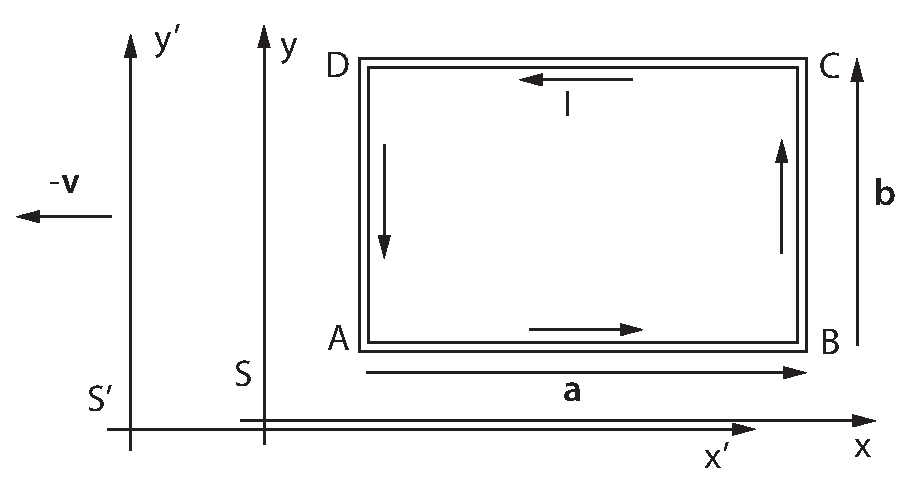
\includegraphics[width=8cm]{currentloop.eps}
\end{center}
\caption{Illustration of current loop. \label{fig:currentloop}}
\end{figure}
%%%%%%%%%% 

\begin{itemize}
\item[{\bf a)}] Show that in the rest frame the loop's electric dipole moment is zero and the magnetic moment is $\vec m=I\vec a\times \vec b$, where $I=j\Delta$ with $j$ as the current density and $\Delta$ as the cross section area of the current wire.
\end{itemize}

In the following we will examine how the loop is observed in a reference frame $S'$, where the loop is moving with velocity $\vec v$ to the right ($\beta=v/c$ and $\gamma=1/\sqrt{1-\beta^2}$). The Lorentz transformation formulas for charge and current denisities may be useful when solving the problems below.

\begin{itemize}
\item[{\bf b)}] What is the length and width of the loop in $S'$?
\item[{\bf c)}]Show that the parts AB and CD of the loop have charge $\pm aIv/c^2$ in $S'$.
\item[{\bf d)}]Show that in $S'$ the loop's electric dipole moment is ${\vec p}'=-\frac{1}{c^2}\vec{m}\times\vec{v}$, and the magnetic dipole moment is $\vec{m}'=(1-\beta^2/2)\vec{m}$.
\item[{\bf e)}]Show that the current  is $I\gamma$ in the AB and CD and $I/\gamma$ in BC and DA.
\item[{\bf f)}]Show that the result in {\bf e)} is consistent with charge conservation.
\end{itemize}
\end{exercise}


%%%%%%%%%%
\begin{exercise}
%%%%%%%%%%
An electric point charge $q$ is moving with constant velocity $\vec v$ along the $x$-axis of the inertial frame $S$, as illustrated in Fig.~\ref{fig:dipole}. Assume it passes the origin of $S$ at $t=0$.

%%%%%%%%%%
\begin{figure}[h]
\begin{center}
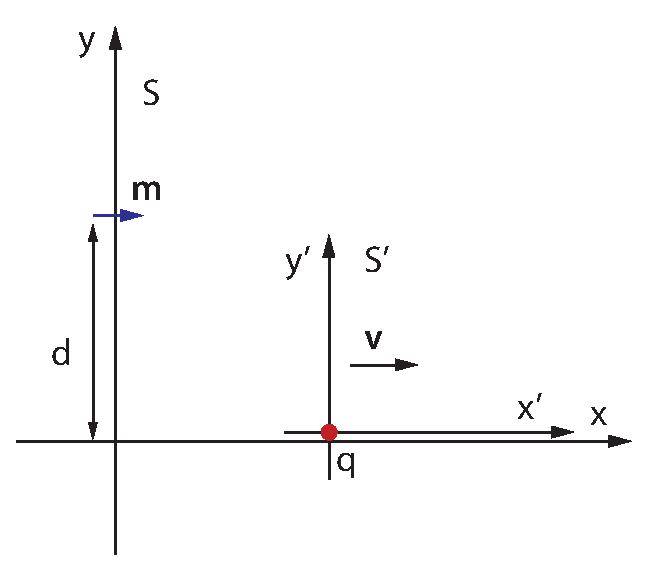
\includegraphics[width=6cm]{dipole.eps}
\end{center}
\caption{Charge on the move. \label{fig:dipole}}
\end{figure}
%%%%%%%%%% 

\begin{itemize}
\item[{\bf a)}] Give the expression for the scalar potential $\phi'$ and the vector potential $\vec A'$ set up by the charge in its rest frame $S'$. In the relativistic description the scalar and vector potentials define the four-potential $A'^\mu$, with the time component related to the scalar potential as $A'^0=\phi'/c$.  Make use of the transformation properties of the four-potential to determine its components $A^\mu$ in reference frame $S$ as functions of the coordinates $(ct, x, y, z)$ in the same frame.
\item[{\bf b)}] Determine (the components of) the electric field  $\vec E$  in the reference frame $S$, as functions of $(ct, x, y, z)$.
\item[{\bf c)}] Determine similarly the magnetic field  $\vec B$  in reference frame $S$.
\end{itemize}

\smallskip
A magnetic dipole, with dipole moment $\vec m$, is at rest in $S$, at the position $(x,y,z)=(0,d,0)$. The dipole vector $\vec m$ points in the $x$-direction.

\begin{itemize}
\item[{\bf d)}] The field from the moving charge acts with a time dependent torque on the dipole, $\vec M=\vec m\times \vec B$. Find the expression for the torque.
\item[{\bf e)}] Assuming the magnetic dipole can be viewed as a small current loop, the force on the dipole from the field produced by the moving charge is $\vec F=\vec\nabla(\vec m\cdot \vec B)$. Determine the force. 
\end{itemize}
\end{exercise}

%%%%%%%%%%
\end{document}
%%%%%%%%%%


